\documentclass{standalone}
\usepackage{tikz}
\usepackage{ctex,siunitx}
\usepackage{tkz-euclide}
\usepackage{amsmath}
\usetikzlibrary{patterns, calc}
\usetikzlibrary {decorations.pathmorphing, decorations.pathreplacing, decorations.shapes,}
\begin{document}
\small
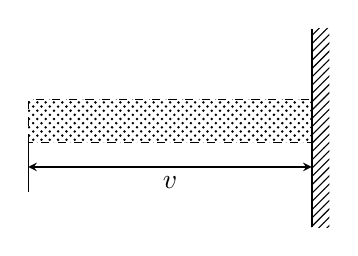
\begin{tikzpicture}[>=stealth,scale=0.9]
  \draw [thick](5,1.3)--(5,-1.5);
  \fill [pattern=north east lines](5,-1.5) rectangle(5.25,1.3);
  \draw[dashed, pattern=crosshatch dots](1,-.3) rectangle (5,.3);
  \draw(1,-.3)--(1,-1);
  \draw[<->](1,-.65)--node [below]{$v$}(5,-.65);
\end{tikzpicture}
\end{document}